\documentclass{amia}
\usepackage{graphicx}
\usepackage[labelfont=bf]{caption}
\usepackage[superscript,nomove]{cite}
\usepackage{color}
\usepackage{multirow}
\renewcommand*{\thefootnote}{\fnsymbol{footnote}}

\begin{document}

\title{Machine Learning Models for the Segmentation of Clinical Exchange}

\author{Mehedi Hasan, BS$^{1}$\footnote[1]{Authors provided equal contribution. \label{footnote1}}, Alexander Kotov, PhD$^{1}$\textsuperscript{\ref{footnote1}}, Ming Dong, PhD$^{1}$, Sylvie Naar, PhD$^{2}$, Gwen L. Alexander, PhD$^{3}$, April Idalski Carcone, PhD$^{4}$}

\institutes{
$^1$Department of Computer Science, Wayne State University, Detroit, Michigan \\  
$^2$Director, Center for Translational Behavioral Research, Department of Behavioral Sciences and Social Medicine, Florida State University, Tallahassee, Florida\\
$^3$Department of Public Health Sciences, Henry Ford Health System, Detroit, Michigan\\
$^4$Department of Family Medicine and Public Health Sciences, School of Medicine, Wayne State University, Detroit, Michigan\\
}

\maketitle

\noindent{\bf Abstract}
\textit{Communication science to understand clinical process like Motivational Interviews (MI) is limited by traditional qualitative coding methods. Qualitative coding of communication data is very resource-intensive and time-consuming process, requires auto coding. This study utilized e-coaching data where email is used to deliver motivation-enhancing coaching to encourage healthy eating. A critical step toward automatic annotation of communication coding process is the segmentation of text data. In this study, we transformed segmentation task into a classification task and developed several state-of-the-art machine learning models including Support Vector Machine, Naive Bayes, K-Nearest Neighbor (KNN), Recurrent Neural Networks by utilizing contextual, topic and punctuation mark features. Results indicate that KNN is the best model and achieved 0.986 F1-measure in overall, 0.779 and 0.993 F1-measures for detecting ``boundary'' and ``not boundary'' classes, respectively. This study has a great implication to save money and accelerate the pace of identifying effective communication strategies.}

\section*{Introduction}
Communication science to understand clinical process like Motivational Interviews (MI) is limited by traditional qualitative coding methods. Motivational Interviewing (MI) is an evidence-based communication technique to increase intrinsic motivation and self-efficacy for behavior change\cite{miller2012motivational,miller2009ten,miller2009toward}. Patient ``change talk'', statements of intrinsic motivation about their desire, ability, reasons, need for and commitment to behavior change, is an established mediator of health behavior change\cite{apodaca2009mechanisms}. Qualitative coding of communication data has been traditionally performed manually with pre-defined codes by trained coders, which is a tedious resource-intensive task, requiring an iterative process of human (subjective) interpretation of the text.   

Rapidly developing computational technologies, specifically, machine learning models, offer a unique opportunity to accelerate this process. Machine learning-based classification methods have been successfully applied to a variety of analytical tasks on textual data including classification\cite{nigam2000text}, sentiment analysis\cite{wang2012baselines}, and digital forensics\cite{de2002language}. A few studies have been done for the automatic annotation of clinical interactions in the setting of MI intervention. Lacson et al.\cite{lacson2005automatic} applied AdaBoost\cite{freund1999short} classifier for annotating the interactions in hemodialysis phone dialog as Clinical, Technical,
Backchannel, and Miscellaneous categories. Our research group has recently applied several machine learning-based models to MI sessions \cite{hasan2016study,kotov2015interpretable}. A simple communication code scheme was automated to characterize patient communication and achieved accuracy comparable to human coders\cite{hasan2016study}. 

Experimental data utilized in the above MI studies were prepared by transcribing audio conversation which involves a counselor, a patient, and some cases a caregiver\cite{hasan2016study,kotov2015interpretable}. However, this study utilized e-coaching data which have different structure and context compared to traditional clinical data. E-coaches use email to deliver motivation-enhancing coaching to encourage healthy eating, grounded in the principles of motivational interviewing. E-coaching data is comprised of email responses which are unsegmented, unlike more traditional dyadic clinical communication where segmentation occurs naturally due to its conversation nature. Discourse analysis on e-coaching text can help to understand the communication process in e-coaching text by revealing the socio-psychological characteristics of a patient\cite{siegfried1995therapeutic,kalchbrenner2013recurrent,pierre2016neural}. By utilizing e-coaching data and leveraging innovative machine learning models, the ultimate goal of this research study is to fully automate the communication coding process.

A significant barrier to fully automated the communication coding process is the segmentation of the text data. During traditional qualitative coding, coders determine where to segment text, that is, where one code ends and another begins. Automatic segmentation of e-coaching intervention sessions is a challenging task due to the 2 important reasons. First, the email is an unstructured text that contains informal email exchange as a non-traditional format. Second, a text segment does not necessarily belong to the entire sentence or collection of sentences. One sentence can be segmented into multiple MI behaviors or several sentences may represent a single MI code. Figure~\ref{fig:text-segment} illustrates the segmentation of an e-coaching email exchange where the first sentence segmented into 2 different MI behaviors. On the other hand, fourth and fifth segments contain 1 and 3 sentences, respectively.  

\begin{figure}[!htb]
    \centering
    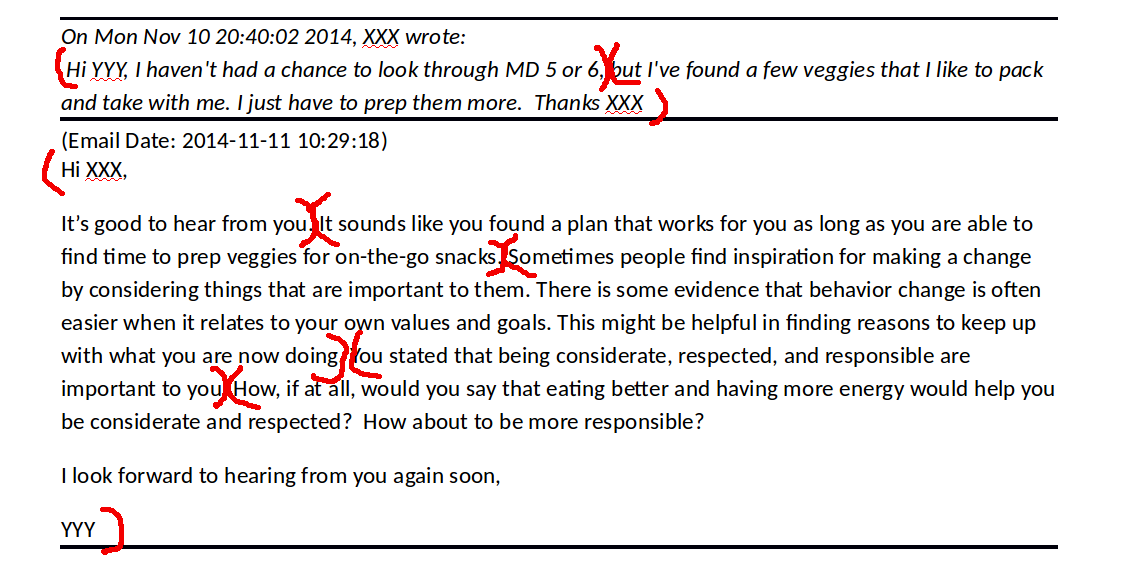
\includegraphics[width=0.9\textwidth]{figures/segment-example.png}
    \caption{\textbf{Segmentation of e-coaching text depicts the main challenges of boundary detection}.}
    \label{fig:text-segment}
\end{figure}

In this paper, we address the text segmentation problem by developing several state-of-the-art machine learning models to promote the automatic identification of best communication strategies without human interference. More specifically, we developed Support Vector Machine (SVM), Naive Bayes (NB), K-Nearest Neighbor (KNN), Long Short Term Memory (LSTM), and Gated Recurrent Unit (GRU) by utilizing contextual, topic and punctuation mark features, to find the best model for the segmentation of e-coaching text. 

Previous studies mainly focus on segmentation of text into sections and headers\cite{apostolova2009automatic,denny2009evaluation,tepper2012statistical,cho2002text} or sentence boundary detection\cite{griffis2016quantitative,kreuzthaler2015detection,treviso2016sentence} in the medical domain. Apostolova et al.\cite{apostolova2009automatic} applied SVM by utilizing word-vector cosine similarity metric combined with several heuristics to classify clinical report into semantic sections such as demographics, history, exam procedure, finding, impression, etc. After identification of each line in the document, Tepper et al. \cite{tepper2012statistical} trained Maximum Entropy models for the section classification. In 2009, Denny et al.\cite{denny2009evaluation} proposed a SecTag algorithm, which combined natural language processing technique, terminology-based rule, and naive Bayesian score for identifying sections and headers that achieved 99\% recall with 95.6\% precision. On the other hand, SVM exploiting with linear kernel and recurrent convolutional neural networks with prosodic, part of speech features and word embeddings, were trained by Kreuzthaler et al.\cite{kreuzthaler2015detection} and Griffis et al.\cite{griffis2016quantitative}, respectively, for the detection of sentence boundary. 

Recently, an online clinical intervention called MENU GenY\cite{alexander2017motivations} (Making Effective Nutrition Choices for Generation Y) was proposed to test its efficacy. MENU GenY is a technology-based public health intervention to encourage increased fruit and vegetable intake among young adult age 21-30, utilized personalized e-coaching data. The goal of MENU GenY was to develop a better coding dictionary among GenY to improve eating habits. However, segmentation of clinical conversation in the context of electronically delivered interventions, in particular, segmentation of clinical interaction text into groups of MI behaviors, is still ignored while relying on manual hand-coded approach. Therefore, this study introduces a novel approach and the authors are not aware of any other work this approach has been considered for the segmentation of e-coaching text.  


\section*{Methods}
\subsection*{\textit{Data collection}}
The experimental dataset for this work was constructed from 49 e-coaching sessions, which include a total of 3,138 segmented and annotated MI behaviors. Each session represents an MI intervention delivered via email. To filter out noise from the dataset, non-ascii characters are removed and then applied stemming to obtain a general form of word from different word representations, such as ``eating'', ``eats'', and ``eat''. We formulate the text segmentation task into a binary classification, as shown in Figure~\ref{fig:classifier}. Clinical exchange is given as the input, it is partitioned as adjacent word pairs by sliding them. Each pair is classified into either ``boundary'' or ``not boundary'' class. The original text is segmented at the position, where an adjacent word pair classified into ``boundary'' class. If all adjacent pairs of a block of text classified into ``not boundary'', the whole block of text is then treated as one segment about a single MI behavior. Totaly, we obtained 95,421 word pairs, which include 3,138 ``boundary'' and 92,283 ``not boundary'' instances.    


\begin{figure}[!htb]
    \centering
    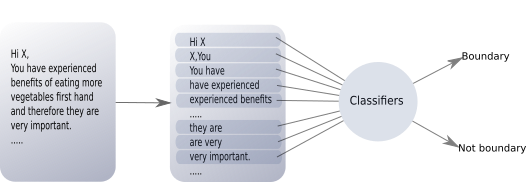
\includegraphics[width=0.80\textwidth]{figures/classifier.png}
    \caption{\textbf{Transformation of text segmentation task into text classification task}.}
    \label{fig:classifier}
\end{figure}


For the experiment, we utilized three type of features including word (textual feature), topic, and punctuation mark. Each word represented in a binary format, where 1 indicates the appearance of the word and 0 for absence. Topics are considered as features since topic models are very effective\cite{kotov2015interpretable,hashimoto2016topic,lu2016modeling} to represent text documents. In this paper, we exploit a topic model named Labeled LDA\cite{ramage2009labeled} model, where topics correspond to labels. The generative process of Labeled LDA drawing the multinomial topic distributions over vocabulary for each topic. In our experiment, we represent each word in a vector of 2 topics, where the number of topics is experimentally determined by the model performance\cite{kotov2015interpretable}. Punctuation mark containing one of the symbols \{`.', `,', `!', `?', `:', `;', `-'\} is also employed as feature. This is one of the most important features as they indicate the boundary of a sentence, clause, and phrase.   

\subsection*{\textit{Segmentation classifiers}}
Several state-of-the-art classifiers, including Naive Bayes (NB)\cite{pedregosa2011scikit}, Support Vector Machine (SVM)\cite{chang2011libsvm}, K-Nearest Neighbor (KNN)\cite{pedregosa2011scikit}, two variant of Recurrent Neural Networks (RNN)\cite{bengio1993problem}: Long Short Term Memory (LSTM)\cite{hochreiter1997long} and Gated Recurrent Unit (GRU)\cite{cho2014properties}, are employed to estimate the classification performance. 

\textbf{Naive Bayes}: this model is constructed by using the training data and estimate the prior probability of classes, and each feature has given the class. Then, the posterior probability is computed to predict the class label by applying the Bayes theorem with the assumption that features are conditionally independent. This study utilized a specialized version of Naive Bayes called Multinomial Naive Bayes, which is best suitable for discrete features such as word.

\textbf{Support Vector Machine}: we used this model as one of the state-of-the-art classification technique proven to perform well in text categorisation\cite{joachims1998text} for its ability to cope with very high dimensional input feature space. SVM finds the best hyperplane in the feature space that maximizes the separation between the closest ``boundary'' and ``not boundary'' training examples. In this experiment, the polynomial kernel is employed to train the SVM model for the segmentation of e-coaching text.   

\textbf{K-Nearest Neighbor}: By this model, each training sample represented as a point in the input feature space. For a new test sample, Euclidean distance is calculated to find the k-nearest neighbors. Finally, the test sample is classified into majority class of the k-nearest neighbors. We experimentally determined that best performance was achieved with k = 3 for the classification of word pairs. 

\textbf{Recurrent Neural Networks}: RNN is a neural network architecture designed to capture sequential patterns present in temporal sequence such as text data. When we predict the ``boundary'' point, adjacent word pair will help to understand the pattern of the sequence. Long Short Term Memory networks usually reffered as LSTMs\cite{hochreiter1997long}, are a special type of RNN capable of handling variable size input sequence, contains internal memory. GRU\cite{cho2014properties} is a variant of LSTM mathematically represented by the following formula:

\begin{equation}
z_t = \sigma(W_zx_t + U_zh_{t-1} + b_z)
\label{eq:firstgru}
\end{equation}
\begin{equation}
r_t = \sigma(W_rx_t + U_rh_{t-1} + b_r)
\label{eq:resetgru}
\end{equation}
\begin{equation}
\tilde h_t = tanh(W_hx_t + r_t \odot U_hh_{t-1} + b_h) 
\label{eq:candidategru}
\end{equation}
\begin{equation}
h_t = z_t \odot h_{t-1} + (1-z_t) \odot \tilde h_t
\label{eq:lastgru}
\end{equation}  
In Eq.~\ref{eq:firstgru}-\ref{eq:lastgru}, $\sigma$ corresponds to sigmoid function and $\odot$ designates an element-wise product. The update gate $z_t$ and reset gate $r_t$ at time step $t$ are computed by the Eq.~(\ref{eq:firstgru}) and~(\ref{eq:resetgru}), where $W_z$, $W_r$, $W_h$, $U_z$, $U_r$, $U_h$ are the weight matrices and $b_z$, $b_h$ and $b_r$ are bias vectors. The activation $h_t$ of the GRU at time $t$ is a linear combination of previous activation $h_{t-1}$ and the candidate activation $\tilde h_t$, which is represented by Eq.~(\ref{eq:lastgru}) and~(\ref{eq:candidategru}). We build our RNN model with one hidden layer, output layer, and input layer. One segmented text was taken as input sequence which get one hot encoding of word vector for the model input. A binary label was assigned as output sequence where ``boundary'' and `not boundary'' words were associated with label 1 and 0, respectively. Since one-hot vector is given in the input layer, results are reported with textual and punctuation mark features only. We experimentally determined that the best performance is achieved when the number of hidden units = 25, batch size = 1, and optimizer = adam.         
  
\subsection*{\textit{Evaluation metrics}}
In this experiment, standard metrics: precision, recall, and F1-measure, are applied to evaluate the performance of binary classifiers\cite{aas1999text}. However, accuracy is not reported as a performance metric because accuracy is highly sensitive to the prior class probabilities and does not fully describe the actual difficulty of the decision problem for an unbalanced dataset. We conduct the experiment with 5 folds cross-validation and weighted macro-averaging of these metrics over the folds. All models have trained on 80\% of the word pairs and remaining 20\% of the data is used as a test set for reporting the performance of the model. We also estimate the area under the receiving operating characteristics (ROC) curve\cite{kumar2011receiver} (AUC) metric due to its effectiveness in measuring the quality of binary classifiers for imbalanced datasets\cite{hu2015kernelized}. 

\section*{Results}
Experimental results are evaluated with ``boundary'' and ``not boundary'' classes as well as their weighted average, which are shown in Table~\ref{tab:result_boundary}, \ref{tab:result_not_boundary}, and \ref{tab:result_weighted_avg}, respectively.\\

\begin{table}[ht]
\centering
\caption{Performance of NB, SVM, KNN, and RNN methods for detecting segmentation boundary in e-coaching text. The highest value for each performance metric is highlighted in bold.}
\label{tab:result_boundary}
  \begin{tabular}{|l|l|l|l|p{0.15\linewidth}|p{0.15\linewidth}|l|}
  \hline
   \multirow{2}{*}{\textbf{Method}} & \multicolumn{3}{|c|}{\textbf{contextual features only}} & \multicolumn{3}{|c|}{\textbf{contextual + punctuation marks (+ topics except RNN)}} \\\cline{2-7}
   & \textbf{Precision}  & \textbf{Recall} & \textbf{F1-measure} & \textbf{Precision}  & \textbf{Recall} & \textbf{F1-measure}\\ \hline    
    
 NB & 0.594 & 0.662 & 0.626 & 0.590 & 0.666 & 0.626 \\ \hline
 SVM & 0.742 & \textbf{0.679} & 0.709 & 0.774 & 0.696 & 0.733\\ \hline
 KNN & \textbf{0.808} & 0.663 & \textbf{0.728} & \textbf{0.820} & \textbf{0.742} & \textbf{0.779}\\ \hline
 LSTM & -- & -- & -- & 0.800 & 0.646 & 0.714  \\ \hline
 GRU & -- & -- & -- & 0.769 & 0.715 & 0.741 \\ \hline 
  \end{tabular}
\end{table}                 

As follows from Table~\ref{tab:result_boundary}, KNN performs best among all machine learning models in terms of precision and F1-measure, achieved 0.808 precision with 0.728 F1-measure when contextual features are used, and 0.820 precision with 0.779 F1-measure when a combination of contextual, topic, and punctuation mark features are used. However, RNN demonstrates the lowest performance among all models in terms of recall and F1-measure while GRU shows 3.72\%, 17.79\% and 11.47\% higher precision, recall, and F1-measure than LSTM. In this study, SVM appears as the second highest model in terms of precision and F1-measure, obtains highest 0.679 recall when only textual features are used. On the other hand, NB exhibits lowest precision value 0.594, provides better recall and F1-measure than RNN model. When textual features are used in combination with topic and punctuation mark features, recall increases by 0.6\%, 2.5\%, and 11.92\%; and F1-measure increases by 0\%, 3.39\%, and 7\% for NB, SVM, and KNN models, respectively. Nevertheless, precision increases by 4.31\% and 1.49\% for SVM and KNN methods while decreases by 0.7\% in NB. \\

\begin{table}[ht]
\centering
\caption{Performance of NB, SVM, KNN, and RNN methods for the identification of ``not boundary'' class. The highest value for each performance metric is highlighted in bold.}
\label{tab:result_not_boundary}
  \begin{tabular}{|l|l|l|l|p{0.15\linewidth}|p{0.15\linewidth}|l|}
  \hline
   \multirow{2}{*}{\textbf{Method}} & \multicolumn{3}{|c|}{\textbf{contextual features only}} & \multicolumn{3}{|c|}{\textbf{contextual + punctuation marks (+ topics except RNN)}} \\\cline{2-7}
   & \textbf{Precision}  & \textbf{Recall} & \textbf{F1-measure} & \textbf{Precision}  & \textbf{Recall} & \textbf{F1-measure}\\ \hline    
    
 NB & 0.988 & 0.985 & 0.987 & 0.989 & 0.984 & 0.986 \\ \hline
 SVM & \textbf{0.989} & 0.992 & 0.991 & 0.990 & 0.993 & 0.991\\ \hline
 KNN & \textbf{0.989} & \textbf{0.995} & \textbf{0.992} & 0.991 & \textbf{0.994} & 0.993\\ \hline
 LSTM & -- & -- & -- & 0.993 & \textbf{0.994} & \textbf{0.994} \\ \hline
 GRU & -- & -- & -- & \textbf{0.994} & \textbf{0.994} & \textbf{0.994} \\ \hline 
  \end{tabular}
\end{table}

Table~\ref{tab:result_not_boundary} summarizes the performance of NB, SVM, KNN, and RNN models for detecting ``not boundary'' class in e-coaching text. We observed that performance is remarkably high in ``not boundary'' class compared to boundary detection which is expected because 96.71\% instances are from ``not boundary'' class. Similar to boundary detection, KNN consistently outperforms over all other methods but obtains 22.40\%, 50.07\%, and 36.26\% higher precision, recall, and F1-measure for contextual features; and 20.85\%, 33.96\%, and 27.47\% higher precision, recall, and F1-measure for combined features compared to boundary class. However, RNN demonstrates the lowest performance and exhibits 0.981 and 0.983 precision with 0.986 and 0.987 F1-measure for LSTM and GRU, respectively. Impact of additional features is also consistent with ``not boundary'' classification. Results show that F1-measure increases by 0\%, and 0.1\% for SVM and KNN models although decreases by 0.1\% for NB. \\

\begin{table}[ht]
\centering
\caption{Weighted average performance of NB, SVM, KNN, and RNN methods for the segmentation of e-coaching text in detecting both ``boundary'' and ``not boundary'' classes. The highest value for each performance metric is highlighted in bold.}
\label{tab:result_weighted_avg}
  \begin{tabular}{|l|l|l|l|p{0.15\linewidth}|p{0.15\linewidth}|l|}
  \hline
   \multirow{2}{*}{\textbf{Method}} & \multicolumn{3}{|c|}{\textbf{contextual features only}} & \multicolumn{3}{|c|}{\textbf{contextual + punctuation marks (+ topics except RNN)}} \\\cline{2-7}
   & \textbf{Precision}  & \textbf{Recall} & \textbf{F1-measure} & \textbf{Precision}  & \textbf{Recall} & \textbf{F1-measure}\\ \hline    
    
 NB & 0.975 & 0.974 & 0.975 & 0.976 & 0.974 & 0.975 \\ \hline
 SVM & 0.981 & 0.982 & 0.981 & 0.983 & 0.983 & 0.983\\ \hline
 KNN & \textbf{0.983} & \textbf{0.984} & 0.983 & \textbf{0.986} & \textbf{0.986} & \textbf{0.986}\\ \hline
 LSTM & -- & -- & -- & \textbf{0.986} & 0.983 & 0.984 \\ \hline
 GRU & -- & -- & -- & \textbf{0.986} & 0.985 & \textbf{0.986} \\ \hline 
  \end{tabular}
\end{table} 

Table~\ref{tab:result_weighted_avg} outlines the weighted average results of the experiment on the models for the segmentation of e-coaching text by classifying them into ``boundary'' and ``not boundary'' classes. Overall, KNN obtains the best performance with all metrics and RNN denotes the lowest performance among all methods. NB and SVM demonstrate moderate performance, obtain precision 0.975 and 0.981; recall 0.974 and 0.982; and F1-measure 0.975 and 0.983 when textual features are used. Influence of the additional features is also consistent as above, precision increases by 0.1\%, 0.2\%, and 0.3\%; recall increases by 0\%, 0.1\%, and 0.2\%; and F1-measure increases by 0\%, 0.2\%, and 0.3\% for NB, SVM, and KNN methods, respectively, when combined features are used.\\

\section*{Discussion}
This study is the first efforts to evaluate the automatic segmentation of e-coaching text. Experimental results indicate that KNN is the best model among all machine learning methods considered for this study. KNN achieved 0.986 F1-measure in overall, 0.779 and 0.993 F1-measures for detecting ``boundary'' and ``not boundary'', respectively. The robust performance of KNN provides the evidence that machine learning models are capable to learn information from clinical exchange. Although the domain of this study was intentionally quite small, we believe that our study is not limited to the e-coaching domain, and it can be successfully applied to other domain as well.

The additional topic and punctuation mark feature made a significant improvement in performance of all machine learning methods. Nearly all cases, the model performs better when contextual features are used in combination with topic and punctuation mark features. This results also mean that segmentation performance might be improved by adding more relevant features including human insight into the problem.       

\begin{figure}[!htb]
    \centering
    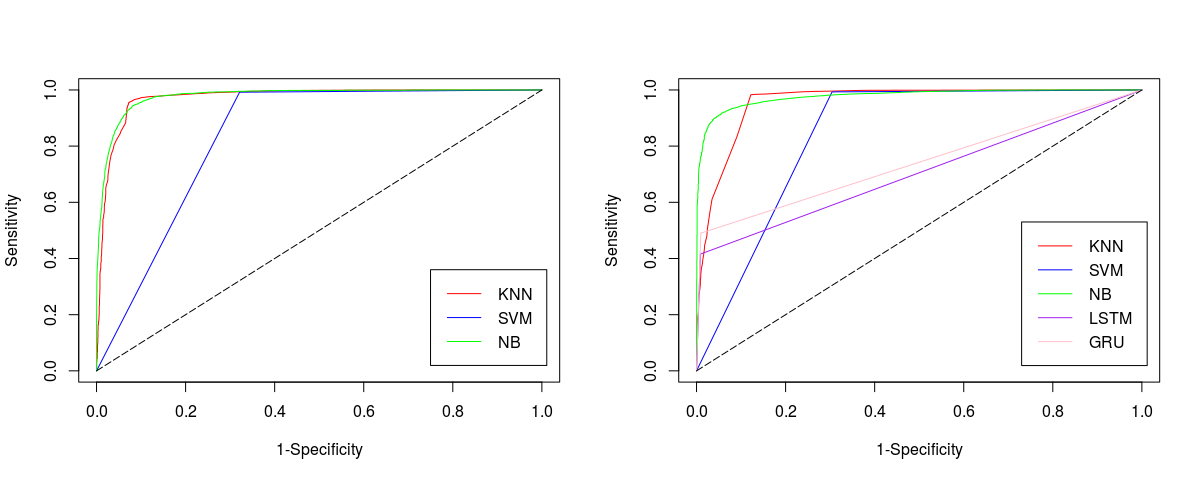
\includegraphics[width=1.0\textwidth]{figures/roc-curves.png}
    \caption{\textbf{Receiver operating characteristic curves showing the performance of binary classifiers for the segmentation of e-coaching text when textual features (left) and combination of textual and other features (right) are used}.}
    \label{fig:roc-curves}
\end{figure}

In this paper, results are reported by each class to avoid confusion about the overall model performance. In addition, standard metrics: precision, recall, and F1-measure were used to eliminate doubt about the model performance because accuracy is misleading for imbalance dataset. AUC values are also outlined due to its effectiveness in measuring the quality of binary classifiers for imbalanced datasets\cite{hu2015kernelized}, which are demonstrated by the ROC curves in Figure~\ref{fig:roc-curves}. NB shows the highest AUC values, achieved 0.978 for both cases while provides lowest classification results. On the other hand, KNN and SVM exhibit 0.972 and 0.835 AUCs when only textual features are used; and 0.959 and 0.844 AUCs when a combination of textual, topic and punctuation mark features are used. Finally, LSTM demonstrates lowest AUC values among all machine learning models, achieved 0.82 AUC while GRU achieved 0.854 AUC. The conclusion drawn from the ROC curves also confirmed the robustness and superiority of KNN model for the segmentation of clinical exchange.      

We observed second highest performance of RNN, in particular, LSTM and GRU for the text segmentation. We believe that RNN will perform better if a large set of data is utilized. In this study, we employed 3,138 examples of boundary case which failed to achieve best results. We also observed that GRU performs better than LSTM which was observed in other previous study\cite{chung2014empirical}.

Although punctuation mark plays an important role in segmentation boundary detection, and large numbers of errors were encountered by the false positive of boundary identification. For example, a text block ``A1 A2 A3. B1 B2 B3. C1 C2 C3 C4.'' can be incorrectly segmented at position A3, B3, and C4 where a punctuation mark was encountered. Similarly, additional information is the common reason for the classified original segment into multiple segments. For instance, the above text block can also be incorrectly segmented at position B3 and C4 because third sentence (C) only supports the MI code confirmed by first two sentences (A and B). 

Our proposed approach is novel for the segmentation of e-coaching text because previous studies mainly focus on the segmentation of text into sections, headers, and sentences in other medical domain. However, this study segmented clinical exchange into groups of MI behaviors which will significantly reduce the amount of resource and time required to segment clinical exchange manually. Furthermore, these segmentation models could be integrated with auto coding classifiers to build a software package of automatic coding procedure of clinical exchange.

The limitation of this study is that e-coaching text is collected from a single medical institute; formatting, style, and email segment can be different in other settings. Therefore, there is a need to replicate the experiments with different data sets. As our future work, we plan to evaluate our approach on other datasets involves in discourse analysis. We also plan to use more relevant features to improve model performance. For example, part-of-speech tagging\cite{hasan2016feedback} and distance from the beginning and end of the current sentence might significantly enhance the classification performance. 
 
\section*{Conclusion}
Segmentation of e-coaching text is an integral part of developing an automated e-coaching intervention. Although several studies have done in clinical interventions, they are limited by the qualitative coding of clinical interactions. In addition, previous studies in the medical domain mainly segmented clinical text into sections and sentences, none of them are used for the segmentation of text into groups of MI behaviors in the setting of discourse analysis with email under the principle of motivational interviews. In this paper, we compared the performance of machine learning models for the task of segmentation of e-coaching text. We found out that k-nearest neighbor provides the best performance for the segmentation of text in terms of all performance metrics. Manual segmentation of e-coaching data is very resource-intensive and time-consuming task, which can significantly decrease the time and effort required to develop an effective behavioral intervention. Our proposed methods can help to identify individual text segments, which can be annotated directly with a classification model. This approach will also help for developing fully automated e-coaching and accelerate the pace of identifying effective communication strategies.

\section*{Acknowledgments}
This study was supported by a grant from the National Institutes of Health, NIDDK R21DK108071, Carcone and Kotov, MPIs. We would like to thank research staff and student assistants in the Department of Family Medicine and Public Health Sciences at Wayne State University School of Medicine for their help in preparing the training dataset. 

\bibliographystyle{vancouver}
\bibliography{references}

\end{document}
